\documentclass{beamer}

\usetheme{JuanLesPins}

\usepackage[utf8]{inputenc}
\usepackage[T1]{fontenc}
\usepackage[french]{babel}
\usepackage[linesnumbered,ruled,french,onelanguage]{algorithm2e}
\usepackage{listings}
\usepackage{color}
\usepackage{pifont}


\definecolor{pblue}{rgb}{0.13,0.13,1}
\definecolor{pgreen}{rgb}{0,0.5,0}
\definecolor{pred}{rgb}{0.9,0,0}

\lstset{language=Java,
  	commentstyle=\color{pgreen},
  	keywordstyle=\color{pblue},
  	stringstyle=\color{pred},
  	basicstyle=\ttfamily,
  	numbers=left,
  	numberstyle=\tiny,
  	basicstyle=\small,
  	frame=single,
  	title=\lstname
}
 
\title{LDVELH-LAP}
\date{25 avril 2022}
\author{Lou-Anne Gautherie, Oumoul Kiramy Bah, Montagne Antonin, Pape Maguette Diongue}
\institute{Université de Caen Normandie}

\setbeamertemplate{navigation symbols}{}% pour enlever les symboles de navigation en bas de chaque page
\setbeamertemplate{footline}[frame number]%pour changer le pied de page par un affichage des numéros de slide

\begin{document}

\maketitle

%--------------------
\begin{frame} 
\frametitle{Plan}
\tableofcontents
\end{frame}
%--------------------
\section{Introduction}
\begin{frame}
\frametitle{Objectif du projet}

\end{frame}
%--------------------
\section{Gestion des nœuds}
\begin{frame}
\frametitle{Description}

\end{frame}
%--------------------
\section{Affichage}
\subsection{Première interface}%à remplir par lou-anne
\begin{frame}
\frametitle{Boutons Accueil / Commencer l'histoire}

\begin{center}
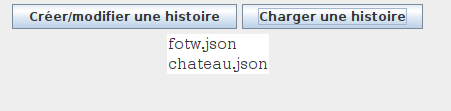
\includegraphics[scale=0.5]{./images/charger.png}\\
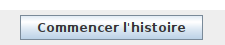
\includegraphics[scale=0.5]{./images/commencer.png}
\end{center}

\end{frame}

\begin{frame}
\frametitle{Mode édition / lecture}

\begin{center}
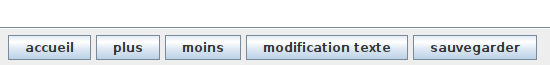
\includegraphics[scale=0.4]{./images/boutonsEdition.png}\\
\vspace{0.6cm}
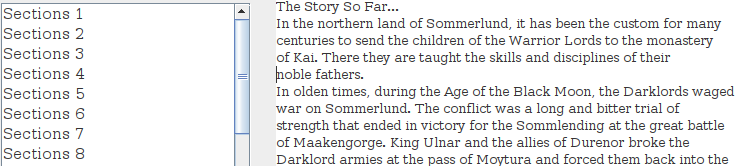
\includegraphics[scale=0.4]{./images/menu.png}\\
\vspace{0.6cm}
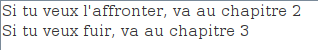
\includegraphics[scale=0.6]{./images/choix.png}
\end{center}

\end{frame}



%--------------------
\subsection{Modes}%à remplir par antonin

\begin{frame}
\frametitle{Actualisation affichage}
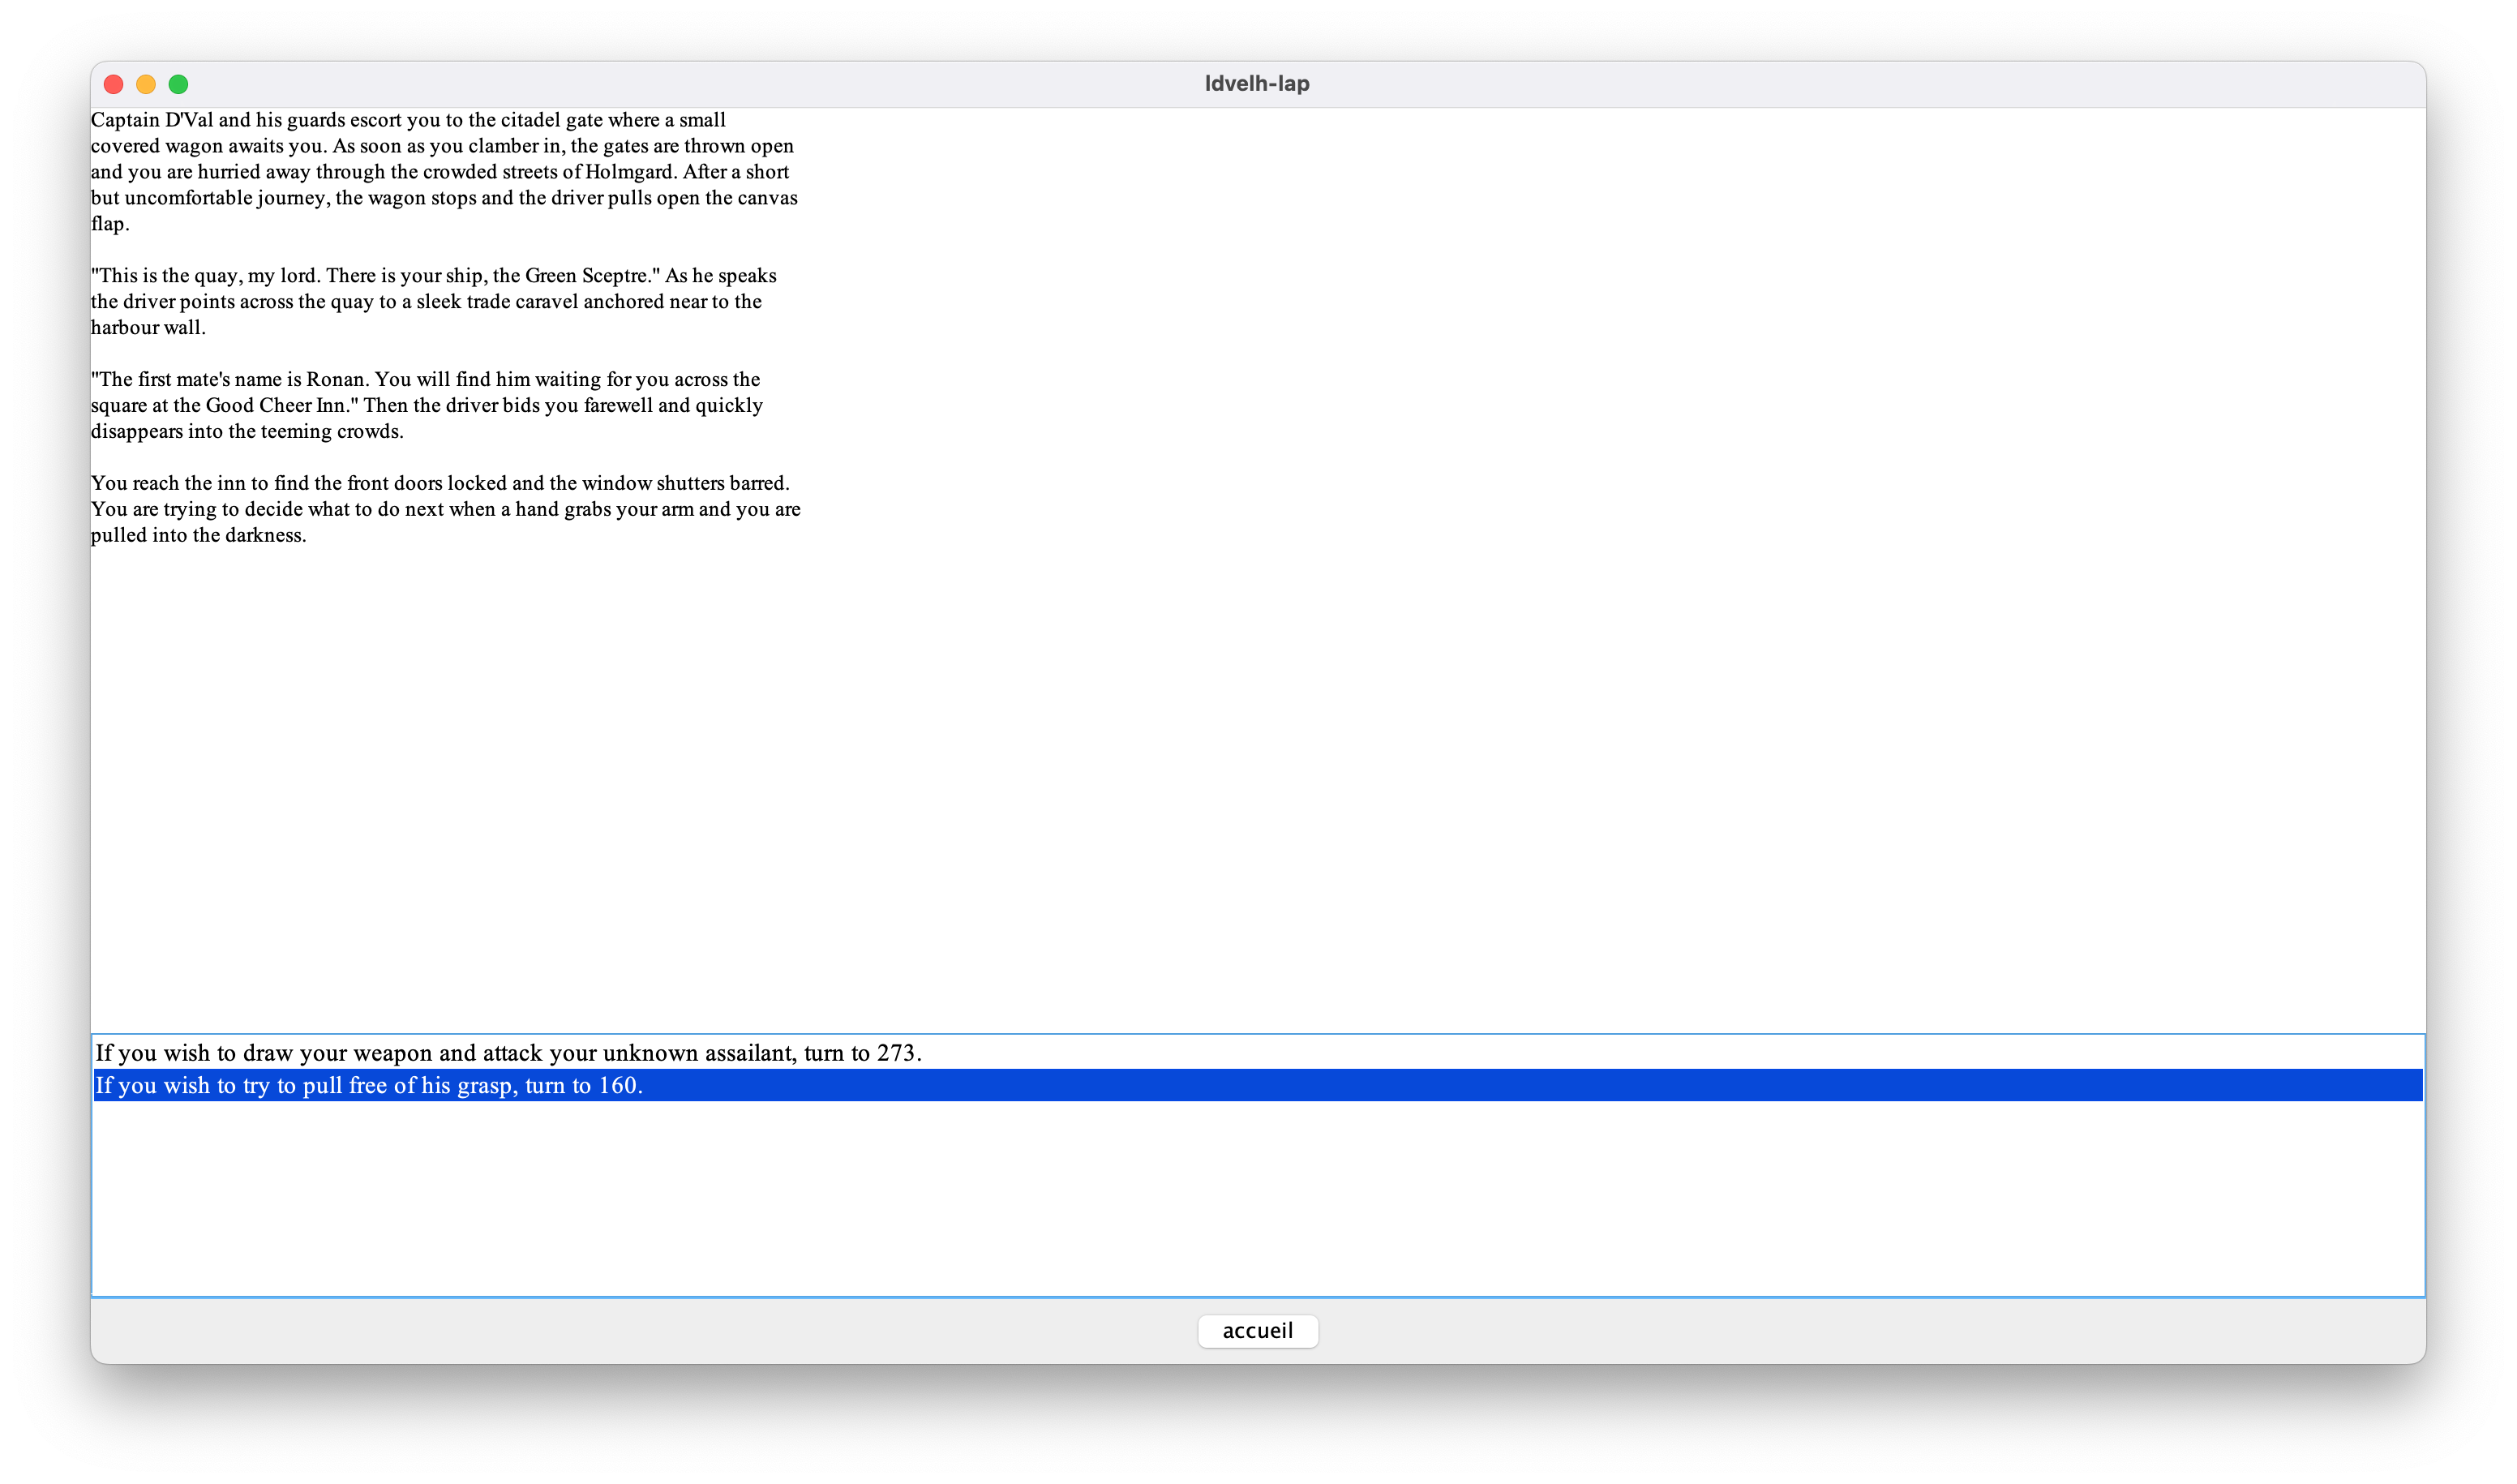
\includegraphics[scale=0.2]{./images/ChoixBug1.png}
\end{frame}

\begin{frame}
\frametitle{Actualisation affichage}
\includegraphics[scale=0.2]{./images/ChoixBug2.png}
\end{frame}

\begin{frame}[containsverbatim]
\frametitle{Actualisation affichage}
\begin{lstlisting}[tabsize=3,gobble=3]
	public void afficherIntro(){
		...
		if(panelPrincipal.getComponentCount()== 2){
			...
			panelMenu.add(scrollPane);
			panelPrincipal.add("West",panelMenu);
			panelPrincipal.add("Center",panelTexte);
			panelPrincipal.add("South",panelBoutons);
		}else{
			panelBoutons.remove(...);
			panelBoutons.remove(...);
			panelBoutons.remove(...);
		}
		...
	}
\end{lstlisting}
\end{frame}

\begin{frame}
\frametitle{Actualisation affichage}
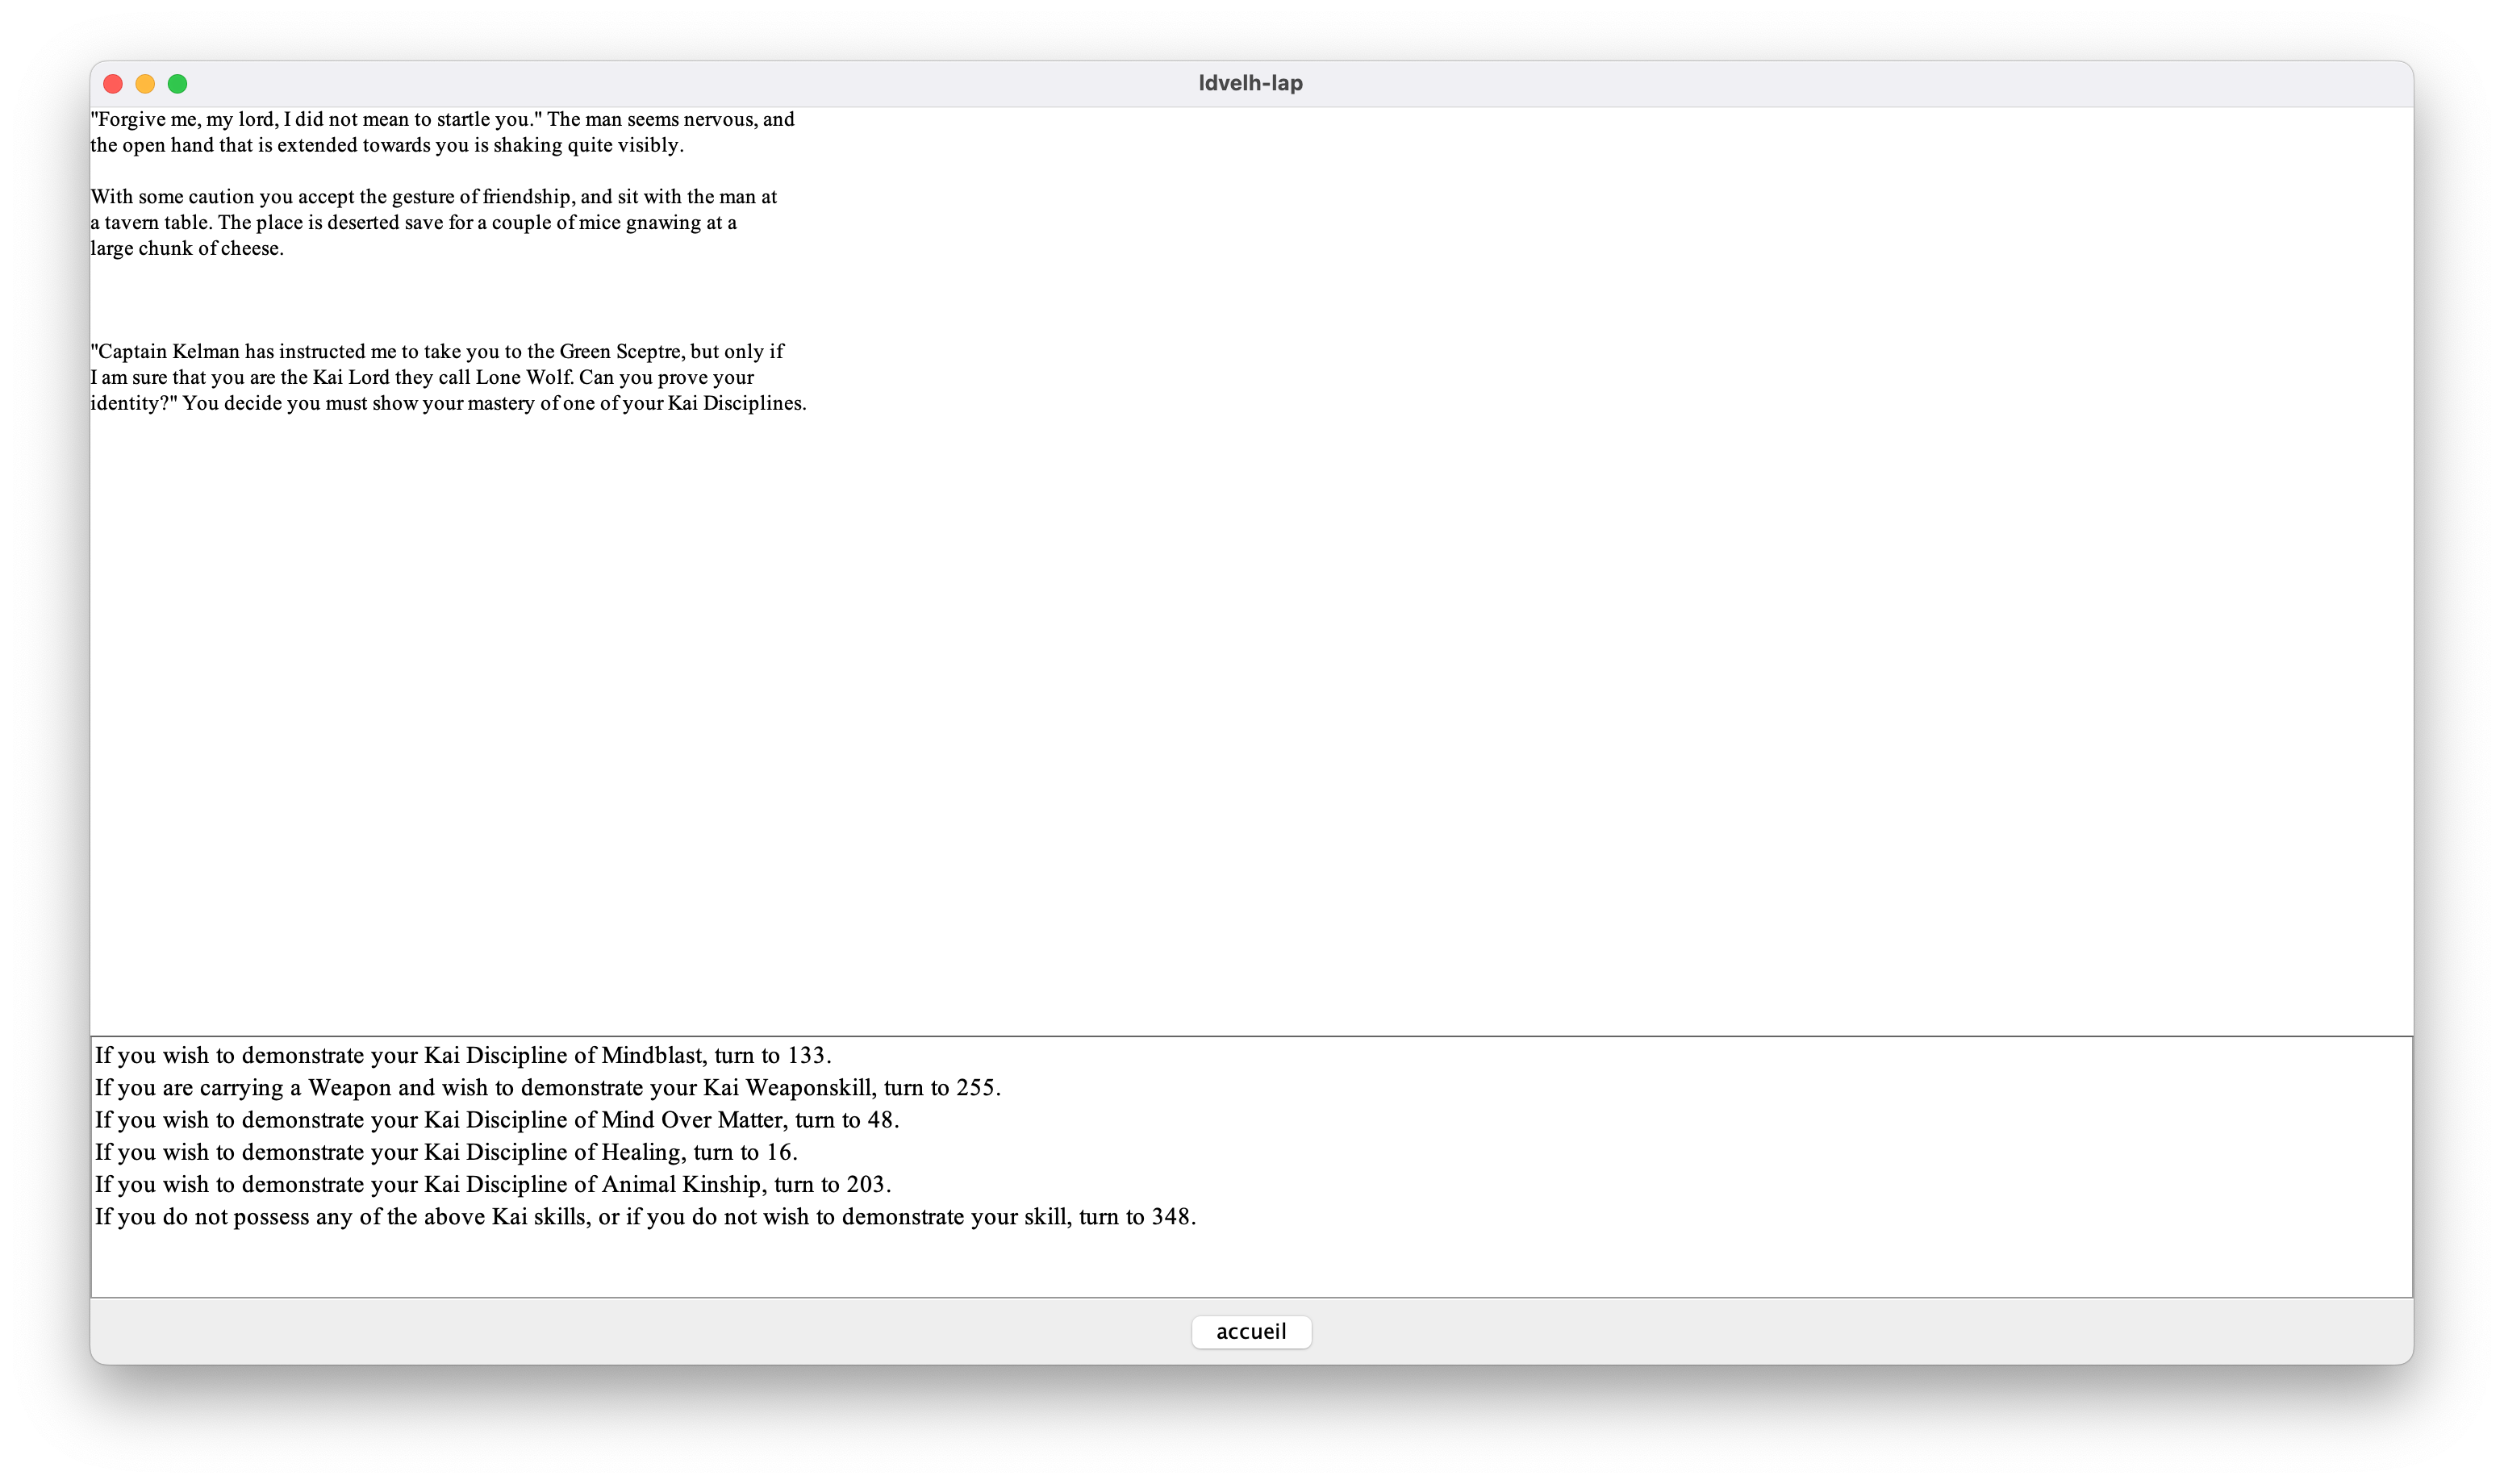
\includegraphics[scale=0.2]{./images/Choix2SansBug.png}
\end{frame}

\begin{frame}[containsverbatim]
\frametitle{Sauvegarde des changements}
\begin{lstlisting}[tabsize=3,gobble=3]
	public void afficherIntro(){
		...
		for(int i = 1; i <= sections.size(); i++){
			modelSections.addElement("Sections " + i);
			HashMap<String,String> vide = new HashMap<>();
			dicoSections.put("Sections " + i, vide);
			String texteVide = "";
			dicoTexteSections.put(i, texteVide);
		}
		...
	}
\end{lstlisting}
\end{frame}

\begin{frame}[containsverbatim]
\frametitle{Sauvegarde des changements}
\begin{lstlisting}[tabsize=3,gobble=3]
   public Sauvegarder(...){
	 for(int i = 1; i <= sections.size(); i++){
      Noeud noeud = new Noeud(...);
      if(dicoTexteSections.get(i).isEmpty()){
       dicoTexteSections.put(...);
       }
       if(dicoSections.get("Sections " + i).isEmpty()){
        HashMap<String,String> mapNoeud = new HashMap(...);
        dicoSections.put(...);
       }
      }
	  ...
	}
\end{lstlisting}
\end{frame}


%-------------------
\section{Graphique}
\begin{frame}
\frametitle{Fichier .dot}

\begin{center}
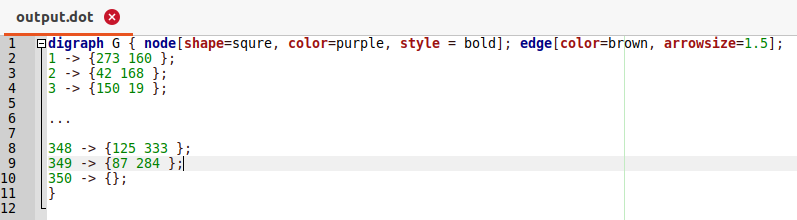
\includegraphics[scale=0.4]{./images/dot.png}
\end{center}

\end{frame}

\begin{frame}
\frametitle{Fichier .png}

\begin{center}
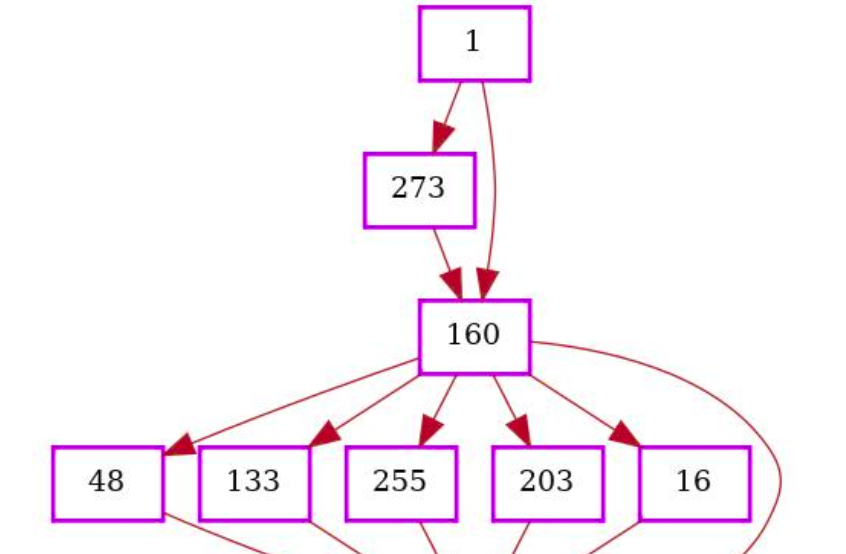
\includegraphics[scale=0.4]{./images/graph.png}
\end{center}

\end{frame}
%--------------------
\section{Tests unitaires}
\begin{frame}
\frametitle{Expérimentations et usages}
\end{frame}
%--------------------
\section{Conclusion}
\begin{frame}
\begin{columns}
\begin{column}{5cm}
Objectifs réalisés
\newline
\begin{itemize}
    \item[\ding{47}] Lire une histoire
 	\item[\ding{47}] Modifier une histoire existante
 	\item[\ding{47}] Créer une nouvelle histoire
 	\item[\ding{47}] Afficher le graphique de l'histoire
\end{itemize}
\end{column}
\begin{column}{4cm}
Fonctions à implémenter
\newline
\begin{itemize}
    \item[\ding{47}] Algorithme de difficulté de l'histoire
 	\item[\ding{47}] Système de rencontre
 	\item[\ding{47}] Combat
\end{itemize}
\end{column}
\end{columns}
\end{frame}


\end{document}
